\subsection*{3.2\quad 人工智能发展脉络}
\noindent 人工智能的发展主线可以从一个朴素问题来理解,那就是知识如何进入系统。早期的做法是把知识写成规则,让机器按规则推理。后来转向从数据中学习统计规律,用泛化能力来应对新情况。再往后是让模型自己学出表示,也就是自动学出特征,从而在更复杂、更开放的环境里保持可扩展性。

\noindent 1955 年达特茅斯提案提出一个关键设想,只要把智能活动写清楚成可执行的规则与流程,机器就能用计算来复现这种能力,并推动 1956 年达特茅斯暑期研讨成为人工智能学科化的起点。此后几十年的几次转向,表面上是算法与工程平台的更替,本质上是知识进入系统的方式在变化。

\begin{figure}[htbp]
\centering
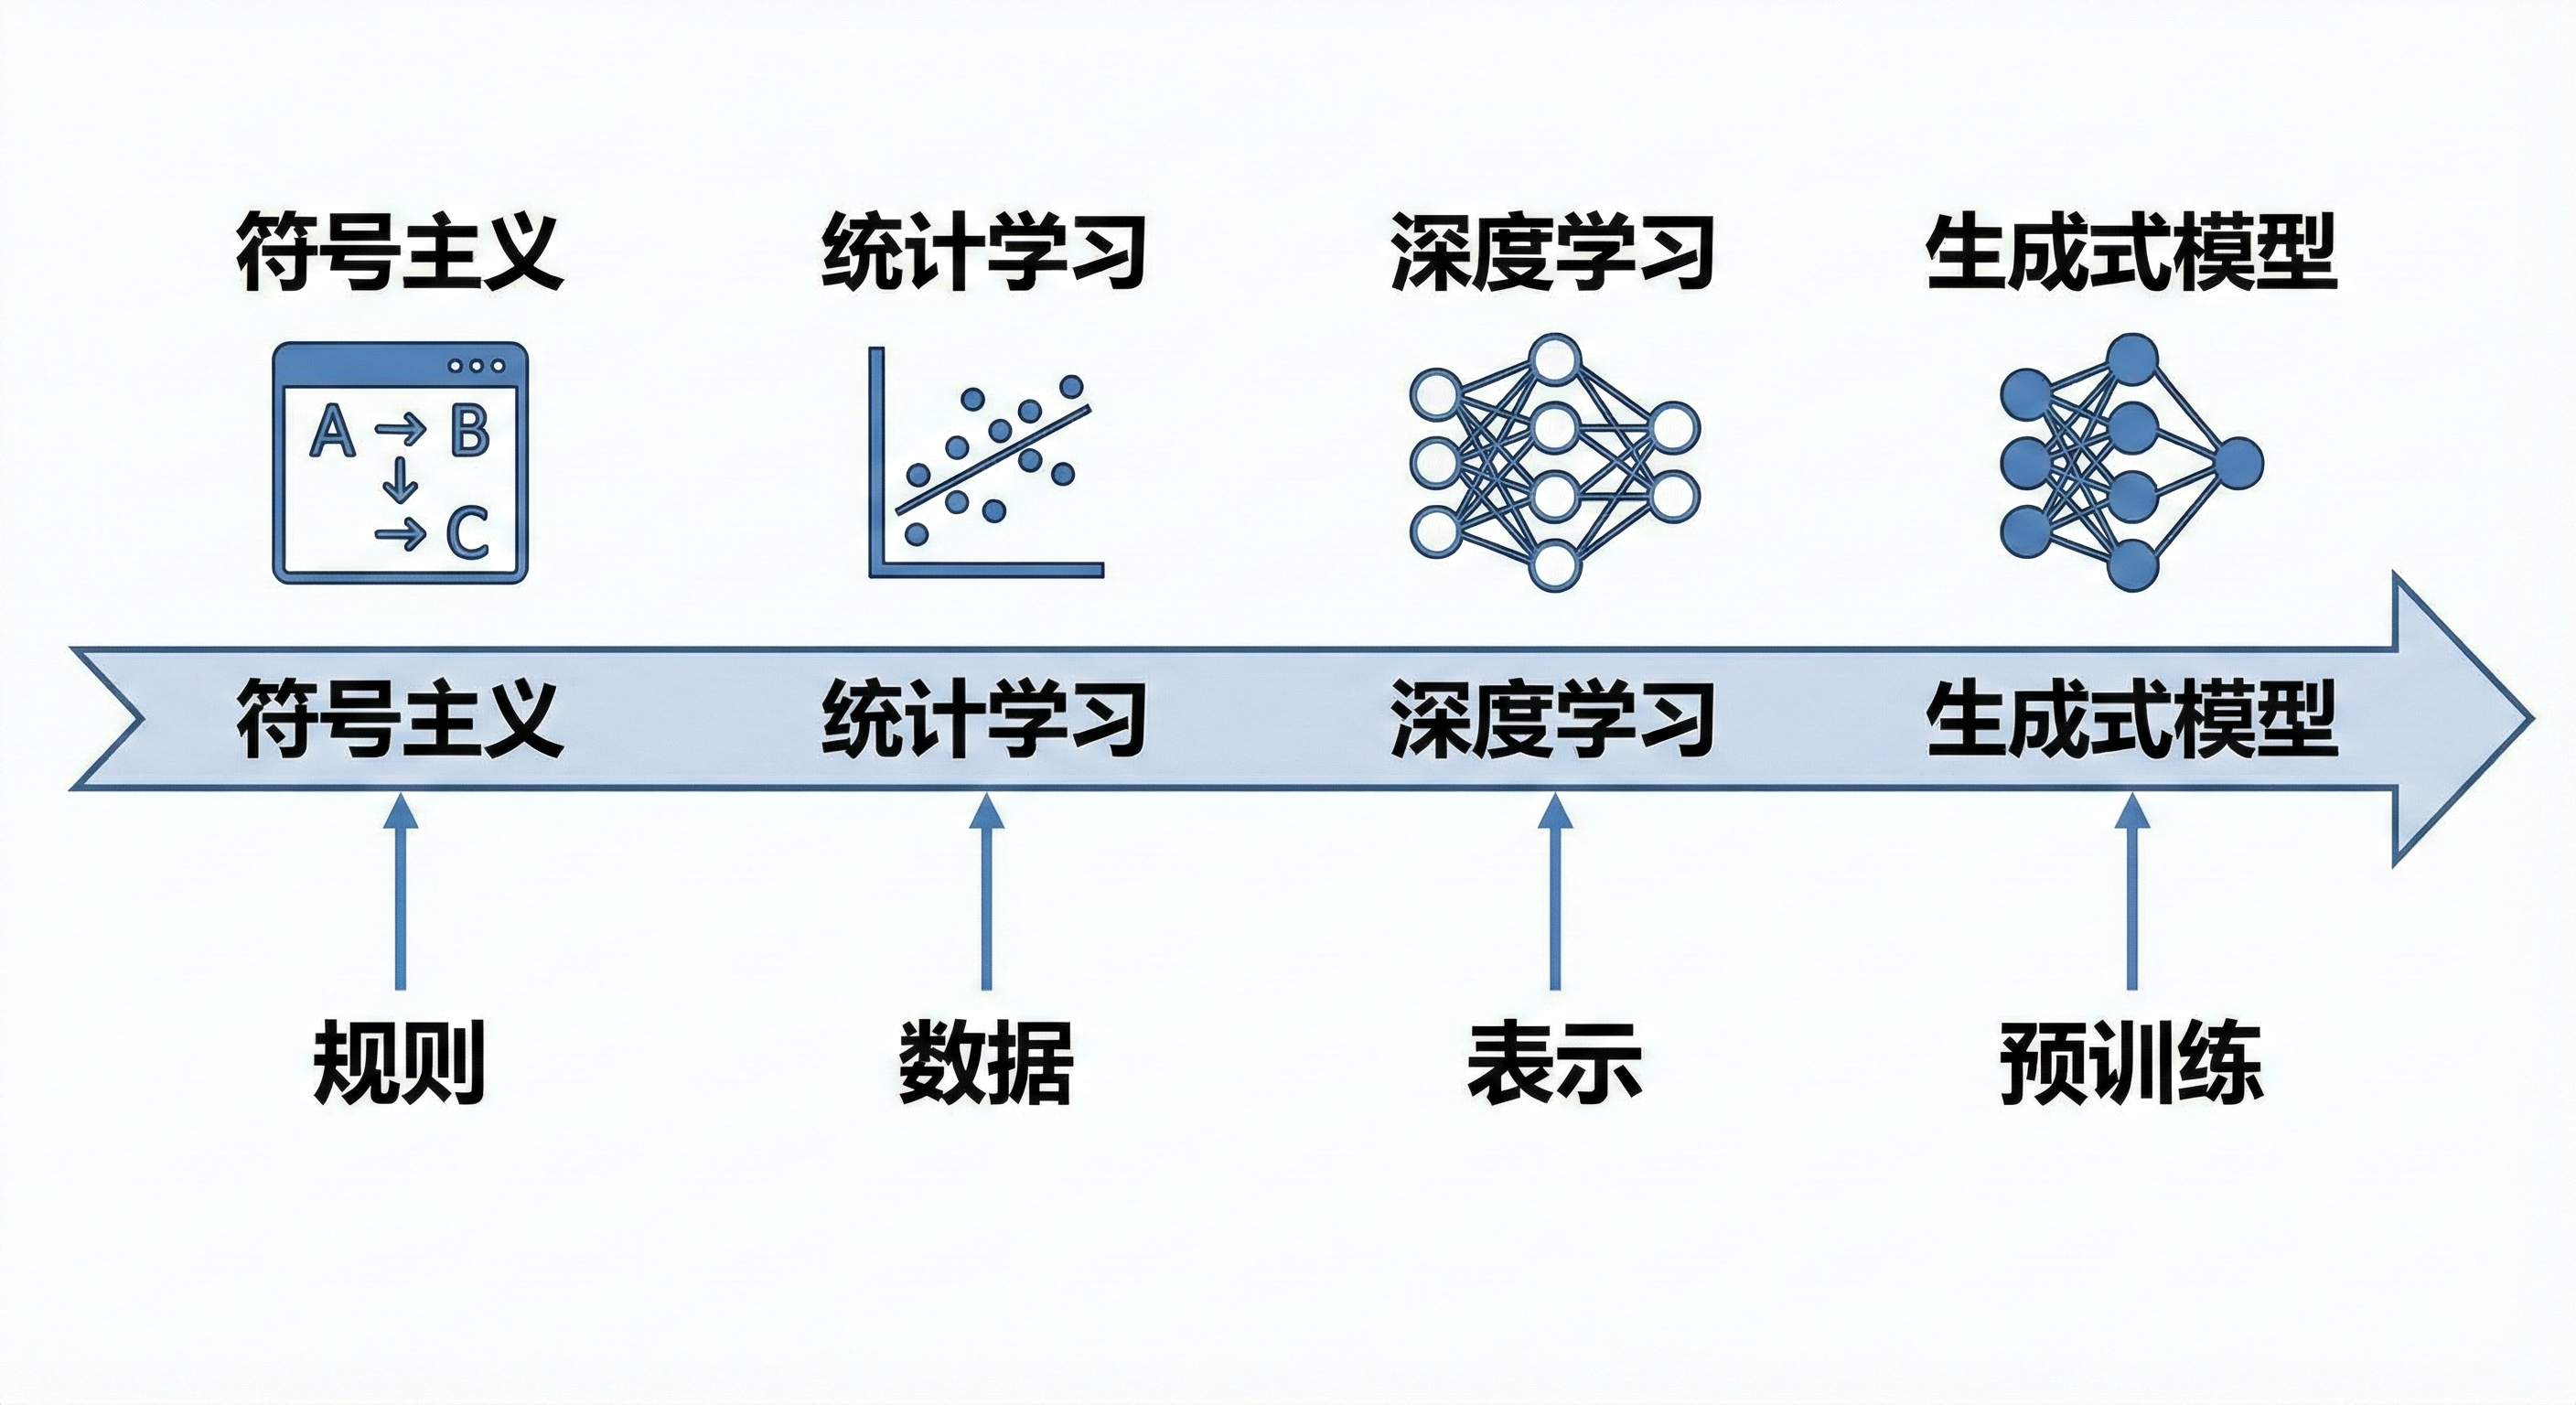
\includegraphics[width=0.9\textwidth]{figures/fig-ai-concept-relation}
\caption{人工智能发展脉络中的概念关系。从符号推理到统计学习,再到深度学习与生成式AI,展示知识进入系统方式的演进。}
\label{fig:ai-concept-relation}
\end{figure}

\subsubsection*{3.2.1\quad 符号推理与专家系统}
\noindent 最早一段时期以符号主义为代表,其核心信念是智能可以被视为符号操作与推理过程。Newell 与 Simon 提出的物理符号系统假说概括了这种立场。只要建立恰当的符号结构与操作规则,就能实现智能行为。

\noindent 在工程实现上,这类系统通常由知识库与推理机构成。知识库保存事实、概念与规则,也包括大量启发式经验法则。推理机通过匹配规则、控制搜索空间、逐步推出结论。专家系统的发展也体现出从纯搜索走向知识工程的路径。相较于只靠搜索,专家系统更强调用知识来聚焦搜索、降低组合爆炸。

\noindent 这解释了为什么符号主义在边界清晰、规则可穷举的问题上表现很好。当你能把什么情况下该怎么做写清楚,系统就能稳定复现专家决策。对乡村经营而言,资格条件清晰的初筛、表单校验、流程分派等任务往往更接近这一类问题,规则体系越稳定,上线后的维护就越可控。

\noindent 但符号主义的天花板同样来自知识进入系统的方式。规则系统的扩展依赖持续加规则,而真实世界的变化会转化为规则库的持续变更,维护成本和一致性问题会迅速放大。以 1980 年代广泛应用的配置型专家系统 XCON 为例,它是典型的规则系统,随着规模增长,规则数在多年运行中膨胀到数千条,并且存在每年大量规则需要变更的维护现实。研究者对其可维护性的评估指出,虽然性能仍可接受,但修改越来越困难。

\noindent 这类问题在组织层面会表现为知识获取瓶颈。系统是否可用越来越取决于能否持续把专家的隐性经验转写成一致、可验证、可演化的规则。一旦维护成本、软硬件成本或预期收益失衡,行业往往进入资金与兴趣收缩的阶段,也就是常说的人工智能寒冬。符号主义不是不聪明,而是其扩展路径太依赖人工编码,难以覆盖开放世界的长尾变化。
\subsubsection*{3.2.2\quad 统计学习与数据驱动方法}
\noindent 统计学习的兴起本质上是在回答同一个难题。规则写不全、写不动时,知识就应当通过数据进入系统。统计学习理论把学习表述为从有限样本进行函数估计并追求泛化,并把控制泛化误差作为核心目标。Vapnik 的工作推动了 1990 年代一批基于该理论的新算法,其中支持向量机成为代表。

\noindent 这一范式的关键变化是如何证明自己在做对的事。模型不再以规则是否符合直觉为主要依据,而是以在未见数据上的表现是否可靠作为硬约束。工程上,这就形成训练、验证、测试分离,交叉验证,指标驱动迭代等方法。算法上,支持向量机等方法用最大间隔与复杂度控制来解释为什么能泛化,在大量结构化任务中成为稳定可用的基线。

\noindent 对乡村经营而言,统计学习更容易嵌入台账与指标体系。只要历史数据口径稳定,目标可以用指标表达,例如需求预测、客流波动预警、信用与风险评分、工单满意度提升等,就可以用数据驱动的方法不断迭代模型,并用上线后的监测与复核机制把风险控制在可接受范围内。
\subsubsection*{3.2.3\quad 深度学习兴起}
\noindent 深度学习的突破进一步推进了知识进入系统的自动化。它不仅减少手写规则,也尽量减少过去必须手工设计的特征,让模型在多层结构中学出表示。其训练机制的关键支点是反向传播。Rumelhart 等人在 1986 年系统描述了通过反向传播不断调整连接权重、最小化输出与目标差异的过程,使多层网络的训练成为可重复的工程方法。

\noindent 但仅有算法并不足以触发行业拐点,竞赛级突破来自数据规模与算力平台的同时成熟。CUDA 在 2007 年正式发布,使 GPU 得以更直接地用于通用并行计算,显著提升了大规模训练的可行性。2012 年 ImageNet 竞赛中,Krizhevsky 等人的深层卷积网络,也常被称为 AlexNet,在一千类、百万级图像数据上取得显著领先,并强调了高效 GPU 卷积实现、非饱和激活等工程选择对训练速度与效果的作用。

\noindent 这次突破的逻辑意义在于,当数据足够大、训练足够快,端到端表示学习可以系统性地超过手工特征加传统分类器的组合,从而改变了计算机视觉等领域的技术路线,并为后续更大规模的预训练模型铺垫方法与工程基础。对乡村经营而言,凡是输入以图片、语音、长文本为主且模式复杂的任务,深度学习更有优势,例如病虫害识别、分级分拣与遥感解译,访谈语音转写与结构化归档,以及政策与材料的要点抽取与归纳。
\subsubsection*{3.2.4\quad 生成式模型与大规模模型概览}
\noindent 在深度学习的基础上,生成式模型与大规模模型把知识进入系统的方式进一步推向大规模预训练。以 Transformer 为代表的架构显著提升了序列建模的并行训练效率,使得在更大规模的数据与参数下训练通用模型成为可行。这类模型通常先在覆盖面很广的文本、图像乃至多模态数据上进行自监督预训练,从而学习到可迁移的通用表示。随后再通过少量示例的上下文提示,也常被称为 in-context learning,或通过面向任务的小规模数据微调,以及更偏工程化的指令化适配,把同一个底座能力迁移到问答、摘要、改写、信息抽取与内容生成等开放任务上。以 GPT-3 为代表的工作系统性展示了规模化预训练对少样本任务迁移能力的提升,即模型在只给少量示例的情况下也能完成多类语言任务。

\noindent 在经营与治理语境下,这类模型更适合承担把材料变成可用文本与可操作线索的工作。例如把分散材料归并成要点,将政策与制度条款转写为可执行清单,对常见问题给出一致口径的问答,辅助形成多版本写作草稿等。与此同时,由于模型输出具有生成性,它并不天然保证事实一致与可追溯,因此需要把可信输入、可引用输出、可核验流程与可追责边界一并设计进系统。一方面在数据来源上建立可追溯的语料与知识库边界,鼓励输出附带依据与引用。另一方面在关键场景引入人工复核、权限控制、日志留存与持续评估等机制,将风险管理纳入全生命周期治理框架。
